% Options for packages loaded elsewhere
\PassOptionsToPackage{unicode}{hyperref}
\PassOptionsToPackage{hyphens}{url}
\PassOptionsToPackage{dvipsnames,svgnames*,x11names*}{xcolor}
%
\documentclass[
]{article}
\usepackage{lmodern}
\usepackage{amsmath}
\usepackage{ifxetex,ifluatex}
\ifnum 0\ifxetex 1\fi\ifluatex 1\fi=0 % if pdftex
  \usepackage[T1]{fontenc}
  \usepackage[utf8]{inputenc}
  \usepackage{textcomp} % provide euro and other symbols
  \usepackage{amssymb}
\else % if luatex or xetex
  \usepackage{unicode-math}
  \defaultfontfeatures{Scale=MatchLowercase}
  \defaultfontfeatures[\rmfamily]{Ligatures=TeX,Scale=1}
  \setmainfont[]{lm}
\fi
% Use upquote if available, for straight quotes in verbatim environments
\IfFileExists{upquote.sty}{\usepackage{upquote}}{}
\IfFileExists{microtype.sty}{% use microtype if available
  \usepackage[]{microtype}
  \UseMicrotypeSet[protrusion]{basicmath} % disable protrusion for tt fonts
}{}
\makeatletter
\@ifundefined{KOMAClassName}{% if non-KOMA class
  \IfFileExists{parskip.sty}{%
    \usepackage{parskip}
  }{% else
    \setlength{\parindent}{0pt}
    \setlength{\parskip}{6pt plus 2pt minus 1pt}}
}{% if KOMA class
  \KOMAoptions{parskip=half}}
\makeatother
\usepackage{xcolor}
\IfFileExists{xurl.sty}{\usepackage{xurl}}{} % add URL line breaks if available
\IfFileExists{bookmark.sty}{\usepackage{bookmark}}{\usepackage{hyperref}}
\hypersetup{
  pdftitle={Behavioural Factors Matter for the Adoption of Climate-Smart Agriculture},
  colorlinks=true,
  linkcolor=Maroon,
  filecolor=Maroon,
  citecolor=Blue,
  urlcolor=Blue,
  pdfcreator={LaTeX via pandoc}}
\urlstyle{same} % disable monospaced font for URLs
\usepackage{longtable,booktabs}
\usepackage{calc} % for calculating minipage widths
% Correct order of tables after \paragraph or \subparagraph
\usepackage{etoolbox}
\makeatletter
\patchcmd\longtable{\par}{\if@noskipsec\mbox{}\fi\par}{}{}
\makeatother
% Allow footnotes in longtable head/foot
\IfFileExists{footnotehyper.sty}{\usepackage{footnotehyper}}{\usepackage{footnote}}
\makesavenoteenv{longtable}
\setlength{\emergencystretch}{3em} % prevent overfull lines
\providecommand{\tightlist}{%
  \setlength{\itemsep}{0pt}\setlength{\parskip}{0pt}}
\setcounter{secnumdepth}{5}
\usepackage[margin=2.8cm]{geometry}
\renewcommand{\contentsname}{Table of Contents}
\usepackage{enumitem}
\usepackage{pifont}
\renewcommand{\labelitemi}{$\rightarrow$}
\usepackage{tocloft}
\renewcommand\cftsecleader{\cftdotfill{\cftdotsep}}
\usepackage{hyperref}
\hypersetup{linkcolor = blue}
\usepackage{hanging}
\usepackage[T1]{fontenc}
\usepackage{graphicx}
\usepackage{booktabs,threeparttablex}
\usepackage{pdflscape}
\usepackage{fvextra}
\DefineVerbatimEnvironment{Highlighting}{Verbatim}{breaklines,commandchars=\\\{\}}
\usepackage{fouriernc}
\usepackage{caption}
\usepackage{nimbusmono}
\usepackage{lscape}
\usepackage{longtable}
\renewcommand{\thetable}{S\arabic{table}}
\renewcommand{\thefigure}{S\arabic{figure}}
\setlength{\cfttabnumwidth}{1cm}
\usepackage{booktabs}
\usepackage{longtable}
\usepackage{array}
\usepackage{multirow}
\usepackage{wrapfig}
\usepackage{float}
\usepackage{colortbl}
\usepackage{pdflscape}
\usepackage{tabu}
\usepackage{threeparttable}
\usepackage{threeparttablex}
\usepackage[normalem]{ulem}
\usepackage{makecell}
\usepackage{xcolor}
\ifluatex
  \usepackage{selnolig}  % disable illegal ligatures
\fi

\title{Behavioural Factors Matter for the Adoption of Climate-Smart Agriculture}
\usepackage{etoolbox}
\makeatletter
\providecommand{\subtitle}[1]{% add subtitle to \maketitle
  \apptocmd{\@title}{\par {\large #1 \par}}{}{}
}
\makeatother
\subtitle{Supplementary Tables}
\date{}

\begin{document}
\maketitle

\newpage
\tableofcontents
\newpage
\listoftables
\newpage

\newpage

\newpage

\newpage

\hypertarget{descriptive-statistics}{%
\section{Descriptive statistics}\label{descriptive-statistics}}

\begingroup\fontsize{8}{10}\selectfont

\begin{ThreePartTable}
\begin{TableNotes}[para]
\item \textit{Note: } 
\item The table above presents summary statistics of some of the regression variables by country. Two-sided t-tests were used for statistical testing, and the corresponding p-values are presented in the last column. The tests performed are Pearsons Chi-squared test for categorical variables and the Wilcoxon rank sum test for continuous variables.
\end{TableNotes}
\begin{longtable}[t]{lccc}
\caption{\label{tab:unnamed-chunk-3}Descriptive statistics by country}\\
\toprule
\textbf{Characteristic} & \textbf{Cameroon}, N = 582 & \textbf{Kenya}, N = 530 & \textbf{p-value}\\
\midrule
\endfirsthead
\caption[]{\label{tab:unnamed-chunk-3}Descriptive statistics by country \textit{(continued)}}\\
\toprule
\textbf{Characteristic} & \textbf{Cameroon}, N = 582 & \textbf{Kenya}, N = 530 & \textbf{p-value}\\
\midrule
\endhead

\endfoot
\bottomrule
\insertTableNotes
\endlastfoot
Crop rotation (1/0) & 403 (69\%) & 223 (42\%) & <0.001\\
Intercropping (1/0) & 380 (65\%) & 220 (42\%) & <0.001\\
Fallowing (1/0) & 355 (61\%) & 90 (17\%) & <0.001\\
Organic soil amendments (1/0) & 207 (36\%) & 133 (25\%) & <0.001\\
Number of CSA adopted &  &  & <0.001\\
\addlinespace
\hspace{1em}0 & 32 (5.5\%) & 139 (26\%) & \\
\hspace{1em}1 & 135 (23\%) & 202 (38\%) & \\
\hspace{1em}2 & 113 (19\%) & 117 (22\%) & \\
\hspace{1em}3 & 224 (38\%) & 58 (11\%) & \\
\hspace{1em}4 & 78 (13\%) & 14 (2.6\%) & \\
\addlinespace
Aspirations & 13.54 (1.65) & 10.95 (0.95) & <0.001\\
Aspiration gap (0-1) & 0.76 (0.22) & 0.69 (0.19) & <0.001\\
Gap squared (0-1) & 0.63 (0.27) & 0.52 (0.24) & <0.001\\
Income (IHS) & 11.74 (1.00) & 9.48 (1.25) & <0.001\\
Off-farm activity (1/0) & 169 (29\%) & 144 (27\%) & 0.5\\
\addlinespace
Household size (num) & 5.0 (4.2) & 5.9 (2.8) & <0.001\\
Credit access (1/0) & 108 (19\%) & 228 (43\%) & <0.001\\
Age of head (years) & 50 (15) & 45 (16) & <0.001\\
Education level &  &  & <0.001\\
\hspace{1em}No formal education & 24 (4.1\%) & 98 (18\%) & \\
\addlinespace
\hspace{1em}Primary Education & 253 (43\%) & 172 (32\%) & \\
\hspace{1em}Secondary Education & 275 (47\%) & 234 (44\%) & \\
\hspace{1em}University Education & 30 (5.2\%) & 26 (4.9\%) & \\
Cooperative membership (1/0) & 109 (19\%) & 133 (25\%) & 0.010\\
Extension access (1/0) & 110 (19\%) & 139 (26\%) & 0.003\\
\addlinespace
Gender of head &  &  & 0.8\\
\hspace{1em}Female & 155 (27\%) & 137 (26\%) & \\
\hspace{1em}Male & 427 (73\%) & 393 (74\%) & \\
Asset index & 0.01 (1.71) & 0.00 (1.85) & 0.8\\*
\multicolumn{4}{l}{\rule{0pt}{1em}\textsuperscript{1} n (\%); Mean (SD)}\\
\multicolumn{4}{l}{\rule{0pt}{1em}\textsuperscript{2} Pearson's Chi-squared test; Wilcoxon rank sum test}\\
\end{longtable}
\end{ThreePartTable}
\endgroup{}

\newpage

\hypertarget{main-regression-tables}{%
\section{Main regression tables}\label{main-regression-tables}}

\begingroup\fontsize{7}{9}\selectfont

\begin{ThreePartTable}
\begin{TableNotes}[para]
\item \textit{Note: } 
\item The table presents the results of OLS regressions between aspirations and CSA practices , with robust standard errors, where the standard errors are clustered. The statistical tests conducted are two-sided t-tests. P-values are denoted in square brackets. The presence of an asterisk (*) above a coefficient indicates that the coefficient is statistically different from zero at a predetermined level of significance (*** p<0.01, ** p<0.05, * p<0.1)
\end{TableNotes}
\begin{longtable}[t]{lrrrr}
\caption{\label{tab:unnamed-chunk-4}Full OLS estimates of the relationship between aspirations and CSA practices}\\
\toprule
variables & Crop rotation (1/0) & Intercropping (1/0) & Fallowing (1/0) & Organic soil amendments (1/0)\\
\midrule
\endfirsthead
\caption[]{\label{tab:unnamed-chunk-4}Full OLS estimates of the relationship between aspirations and CSA practices \textit{(continued)}}\\
\toprule
variables & Crop rotation (1/0) & Intercropping (1/0) & Fallowing (1/0) & Organic soil amendments (1/0)\\
\midrule
\endhead

\endfoot
\bottomrule
\insertTableNotes
\endlastfoot
Aspirations & 0.024** & -0.021 & 0.005 & 0.029**\\
 & (0.010) & (0.014) & (0.009) & (0.012)\\
 & {}[0.019] & {}[0.133] & {}[0.605] & {}[0.022]\\
Off-farm activity (1\/0) & 0.036 & -0.048 & 0.026 & -0.032\\
 & (0.037) & (0.039) & (0.032) & (0.032)\\
 & {}[0.338] & {}[0.225] & {}[0.420] & {}[0.317]\\
Household size (num) & 0.006 & 0.004 & 0.001 & 0.001\\
 & (0.004) & (0.005) & (0.004) & (0.004)\\
 & {}[0.155] & {}[0.346] & {}[0.699] & {}[0.773]\\
Credit access (1\/0) & 0.119*** & 0.060* & 0.031 & 0.009\\
 & (0.036) & (0.031) & (0.031) & (0.036)\\
 & {}[0.001] & {}[0.061] & {}[0.314] & {}[0.798]\\
Age of head (years) & 0.000 & 0.000 & -0.001 & -0.002\\
 & (0.001) & (0.001) & (0.001) & (0.001)\\
 & {}[0.807] & {}[0.879] & {}[0.601] & {}[0.189]\\
Educational level (years) & -0.002 & 0.001 & -0.006* & -0.006\\
 & (0.004) & (0.005) & (0.003) & (0.004)\\
 & {}[0.654] & {}[0.904] & {}[0.071] & {}[0.153]\\
Cooperative membership (1\/0) & 0.039 & 0.028 & 0.041 & 0.019\\
 & (0.037) & (0.036) & (0.033) & (0.035)\\
 & {}[0.292] & {}[0.436] & {}[0.217] & {}[0.584]\\
Extension access (1\/0) & 0.085** & 0.071* & -0.005 & 0.046\\
 & (0.041) & (0.040) & (0.033) & (0.031)\\
 & {}[0.043] & {}[0.077] & {}[0.877] & {}[0.139]\\
Head is male (1\/0) & 0.009 & 0.025 & -0.014 & 0.001\\
 & (0.031) & (0.039) & (0.028) & (0.030)\\
 & {}[0.780] & {}[0.523] & {}[0.616] & {}[0.974]\\
Asset index & 0.035*** & -0.012 & 0.038*** & 0.034***\\
 & (0.012) & (0.017) & (0.011) & (0.013)\\
 & {}[0.006] & {}[0.489] & {}[0.001] & {}[0.008]\\
Observations & 1,112 & 1,112 & 1,112 & 1,112\\
R-squared & 0.342 & 0.239 & 0.388 & 0.226\\
F test & 5.748 & 1.653 & 2.606 & 3.905\\*
\end{longtable}
\end{ThreePartTable}
\endgroup{}

\newpage

\begingroup\fontsize{7}{9}\selectfont

\begin{ThreePartTable}
\begin{TableNotes}[para]
\item \textit{Note: } 
\item The table presents the results of OLS regressions between aspirations failure and CSA practices. Robust standard errors are in brackates. The statistical tests conducted are two-sided t-tests. P-values, denoted in square brackets. The presence of an asterisk (*) above a coefficient indicates that the coefficient is statistically different from zero at a predetermined level of significance (*** p<0.01, ** p<0.05, * p<0.1).
\end{TableNotes}
\begin{longtable}[t]{lrrrr}
\caption{\label{tab:unnamed-chunk-5}Full OLS estimates of the relationship between aspirations failure and adoption of CSA practices}\\
\toprule
variables & Crop rotation (1/0) & Intercropping (1/0) & Fallowing (1/0) & Organic soil amendments (1/0)\\
\midrule
\endfirsthead
\caption[]{\label{tab:unnamed-chunk-5}Full OLS estimates of the relationship between aspirations failure and adoption of CSA practices \textit{(continued)}}\\
\toprule
variables & Crop rotation (1/0) & Intercropping (1/0) & Fallowing (1/0) & Organic soil amendments (1/0)\\
\midrule
\endhead

\endfoot
\bottomrule
\insertTableNotes
\endlastfoot
Aspiration gap (0-1) & 0.569** & 1.218*** & 0.631** & 0.419\\
 & (0.271) & (0.325) & (0.250) & (0.266)\\
 & {}[0.040] & {}[0.000] & {}[0.014] & {}[0.120]\\
Gap squared (0-1) & -0.456* & -1.208*** & -0.530** & -0.291\\
 & (0.244) & (0.294) & (0.212) & (0.227)\\
 & {}[0.065] & {}[0.000] & {}[0.015] & {}[0.204]\\
Off-farm activity (1\/0) & 0.036 & -0.064* & 0.024 & -0.029\\
 & (0.038) & (0.038) & (0.033) & (0.032)\\
 & {}[0.352] & {}[0.097] & {}[0.480] & {}[0.363]\\
Household size (num) & 0.006 & 0.004 & 0.002 & 0.002\\
 & (0.004) & (0.004) & (0.004) & (0.004)\\
 & {}[0.130] & {}[0.308] & {}[0.659] & {}[0.715]\\
Credit access (1\/0) & 0.117*** & 0.057* & 0.030 & 0.007\\
 & (0.036) & (0.032) & (0.031) & (0.036)\\
 & {}[0.002] & {}[0.083] & {}[0.338] & {}[0.843]\\
Age of head (years) & 0.000 & 0.000 & -0.001 & -0.002\\
 & (0.001) & (0.001) & (0.001) & (0.001)\\
 & {}[0.947] & {}[0.990] & {}[0.550] & {}[0.153]\\
Educational level (years) & -0.001 & -0.001 & -0.006* & -0.005\\
 & (0.004) & (0.005) & (0.003) & (0.004)\\
 & {}[0.789] & {}[0.840] & {}[0.071] & {}[0.223]\\
Cooperative membership (1\/0) & 0.035 & 0.009 & 0.036 & 0.018\\
 & (0.037) & (0.035) & (0.031) & (0.035)\\
 & {}[0.348] & {}[0.804] & {}[0.254] & {}[0.596]\\
Extension access (1\/0) & 0.086** & 0.078* & -0.004 & 0.045\\
 & (0.041) & (0.040) & (0.033) & (0.031)\\
 & {}[0.041] & {}[0.053] & {}[0.893] & {}[0.142]\\
Head is male (1\/0) & 0.008 & 0.012 & -0.018 & 0.002\\
 & (0.031) & (0.039) & (0.028) & (0.030)\\
 & {}[0.802] & {}[0.754] & {}[0.532] & {}[0.943]\\
Asset index & 0.039*** & -0.016 & 0.039*** & 0.039***\\
 & (0.012) & (0.016) & (0.011) & (0.012)\\
 & {}[0.002] & {}[0.334] & {}[0.001] & {}[0.002]\\
Observations & 1,112 & 1,112 & 1,112 & 1,112\\
R-squared & 0.341 & 0.262 & 0.392 & 0.222\\
F test & 6.342 & 3.600 & 2.849 & 3.614\\*
\end{longtable}
\end{ThreePartTable}
\endgroup{}

\% Please add the following required packages to your document preamble:

\% Note: It may be necessary to compile the document several times to get a multi-page table to line up properly

\begin{landscape}
\begin{longtable}[c]{@{}lrrrr@{}}
\caption{U-shaped tests of aspiration failure }
\label{tab:my-table}\\
\toprule
\textbf{} &
  \multicolumn{1}{l}{\textbf{Crop rotation}} &
  \multicolumn{1}{l}{\textbf{Intercropping}} &
  \multicolumn{1}{l}{\textbf{Fallowing}} &
  \multicolumn{1}{l}{\textbf{OSA}} \\* \midrule
\endfirsthead
%
\endhead
%
\bottomrule
\endfoot
%
\endlastfoot
%
\multicolumn{5}{c}{\textbf{{[}A{]} Pooled}}                                                                       \\* \midrule
Turning point                      & 0.623            & 0.504              & 0.595             & 0.718            \\
Sasabuchi p-value                  & 0.071            & \textless{}0.001   & 0.016             & 0.215            \\
Slope at minimum                   & 0.568            & 1.218              & 0.631             & 0.418            \\
Slope at maximum                   & -0.344           & -1.196             & -0.428            & -0.163           \\
Fieller 95\% confidence   interval & {[}-Inf; +Inf{]} & {[}0.419; 0.569{]} & {[}0.427; 0.86{]} & {[}-Inf; +Inf{]} \\* \midrule
\multicolumn{5}{c}{\textbf{{[}B{]} Cameroon}}                                                                     \\* \midrule
Turning point                      & 0.515            & 0.494              & 0.507             & 0.604            \\
Sasabuchi p-value                  & 0.067            & 0.002              & 0.019             & 0.169            \\
Slope at minimum                   & 0.509            & 1.126              & 0.676             & 0.363            \\
Slope at maximum                   & -0.478           & -1.149             & -0.656            & -0.238           \\
Fieller 95\% confidence   interval & {[}-Inf; +Inf{]} & {[}0.356; 0.577{]} & {[}0.21; 0.834{]} & {[}-Inf; +Inf{]} \\* \midrule
\multicolumn{5}{c}{\textbf{{[}C{]} Kenya}}                                                                        \\* \midrule
Turning point                      & 0.7              & 0.555              & 0.803             & 0.696            \\
Sasabuchi p-value                  & 0.142            & 0.054              & 0.267             & 0.229            \\
Slope at minimum                   & 0.916            & 0.897              & 0.555             & 0.717            \\
Slope at maximum                   & -0.392           & -0.716             & -0.136            & -0.312           \\
Fieller 95\% confidence   interval & {[}-Inf; +Inf{]} & {[}-Inf; +Inf{]}   & {[}-Inf; +Inf{]}  & {[}-Inf; +Inf{]} \\* \bottomrule
\end{longtable}
\end{landscape}
\newpage

\hypertarget{semi-parametric-estimations-of-aspiration-failure}{%
\subsection{Semi-parametric estimations of aspiration failure}\label{semi-parametric-estimations-of-aspiration-failure}}

\begin{figure}[htbp]
\centering
\caption{Loess smoothed relationship between Practice and Gap for each level of CSA}
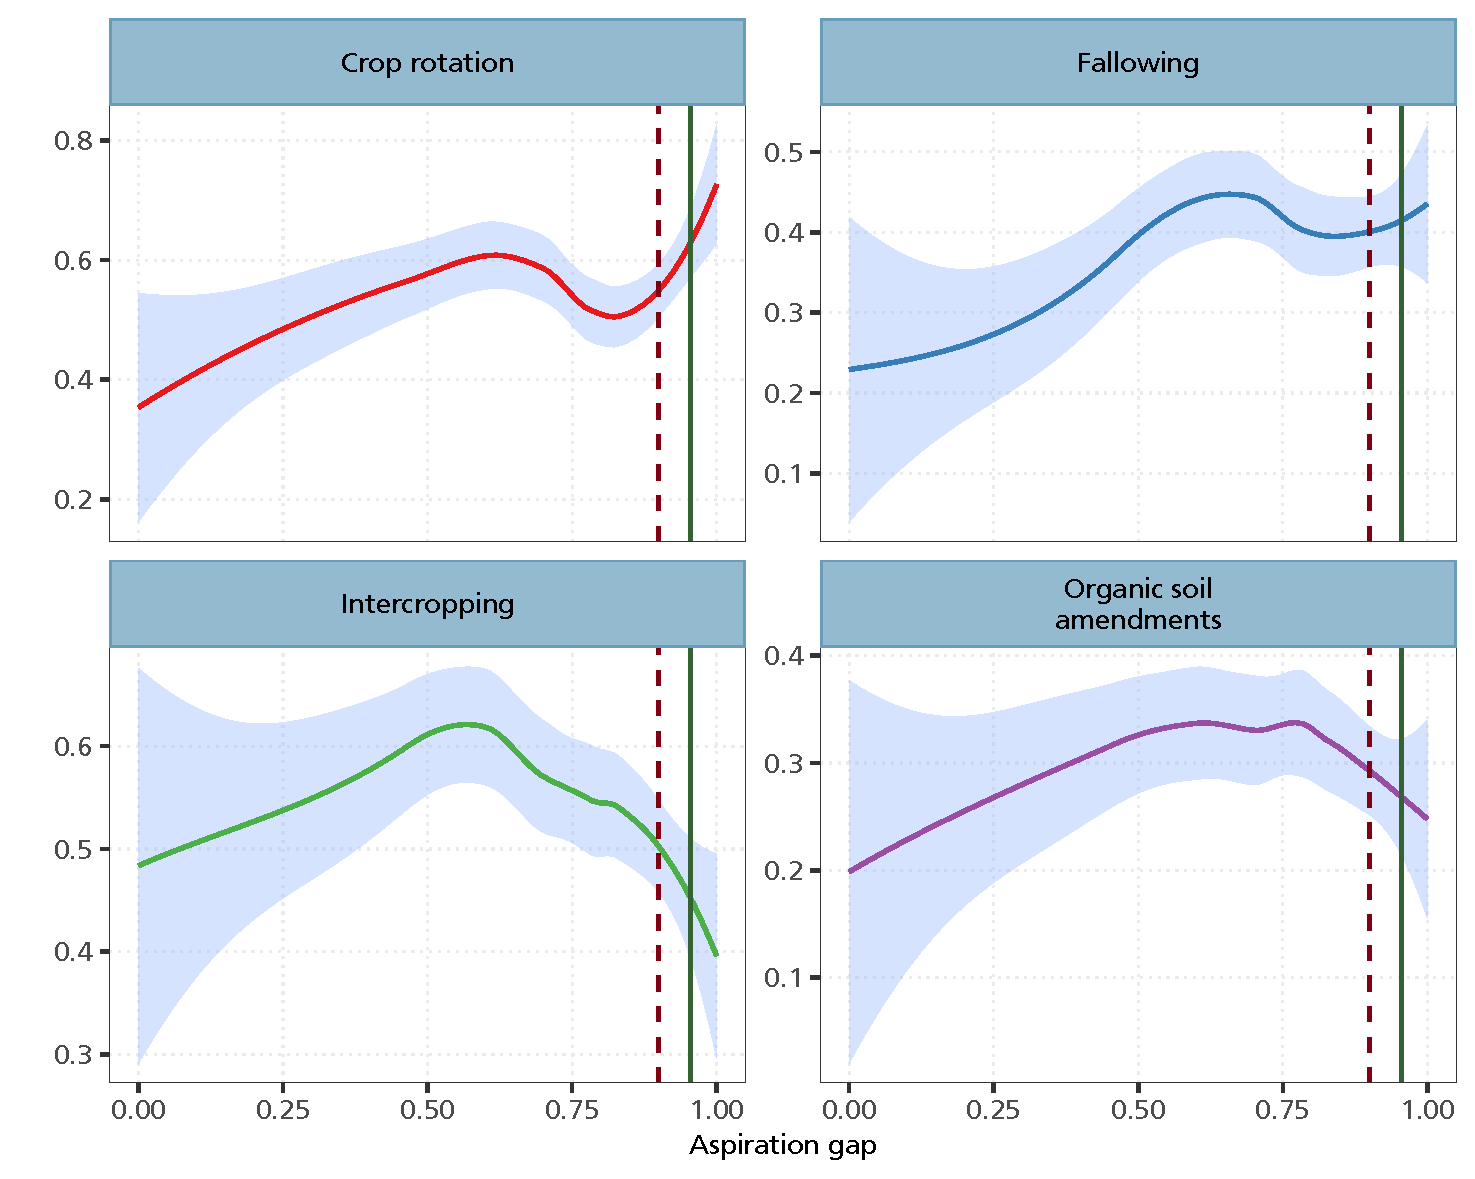
\includegraphics[width=\textwidth]{figures/fig_NP.pdf}

\caption*{
Note: The graph illustrates the relationship between the CSA and Aspiration Gap, stratified by the four different practices.The solid line on each plot depicts a Loess smoothed relationship between aspiration gap and 
practices. Loess smoothing is a nonparametric method that uses local weighted regression to fit a smooth curve through points in a scatter plot. This line represents the trend of CSA adoption as aspiration gap changes. The shaded region around the Loess line represents 95\% Confidence intervals. The red dashed line indicates the 75th percentile, and the green line represents the 90th percentile of the aspiration gap. This figure is derived from a locally weighted regression analysis with a span (alpha) of 0.8 and a polynomial degree of 0.
}
\end{figure}

\newpage

\hypertarget{cameroon}{%
\subsection{Cameroon}\label{cameroon}}

\begin{figure}[htbp]
\centering
\caption{Loess smoothed relationship between Practice and Gap for each level of CSA (Cameroon)}
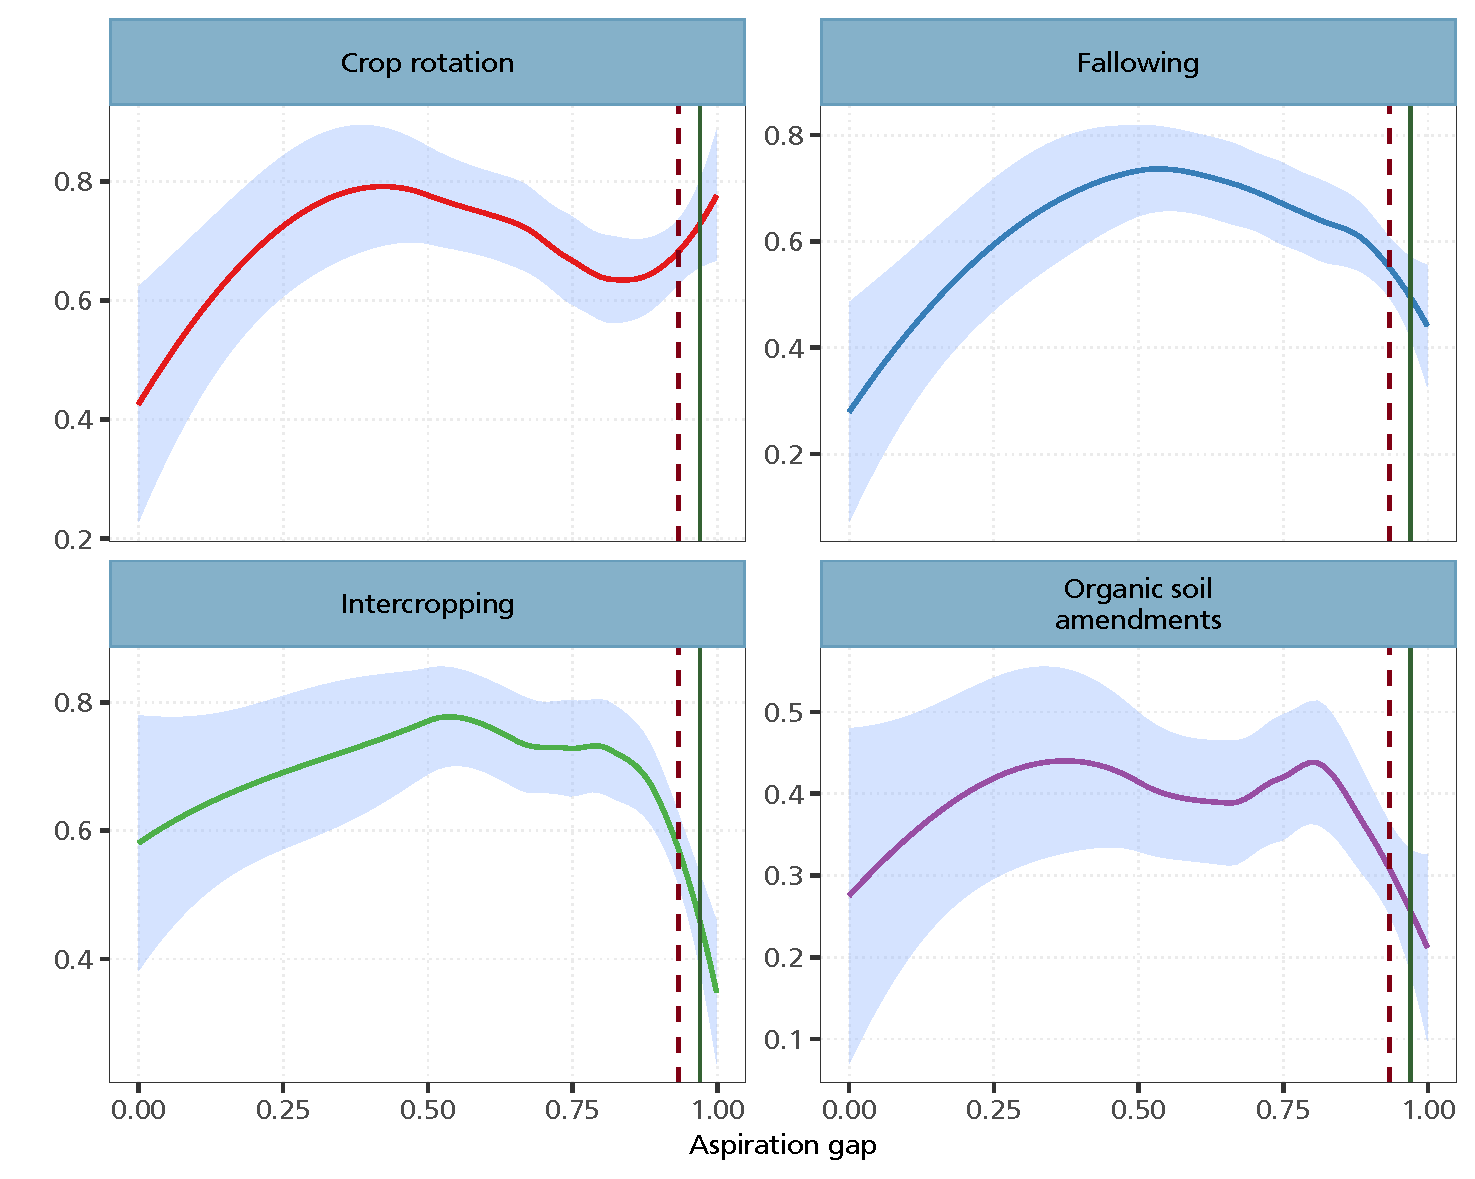
\includegraphics[width=\textwidth]{figures/fig_NP_cam.pdf}

\caption*{
Note: The graph illustrates the relationship between the variable CSA and Aspiration Gap, stratified by the four different practices for Cameroon.The solid line on each plot depicts a Loess smoothed relationship between aspiration gap and CSA practices. Loess smoothing is a nonparametric method that uses local weighted regression to fit a smooth curve through points in a scatter plot. This line represents the trend of CSA adoption as aspiration gap changes. The shaded region around the Loess line represents 95\% Confidence intervals. The red dashed line indicates the 75th percentile, and the green line represents the 90th percentile of the aspiration gap. This figure is derived from a locally weighted regression analysis with a span (alpha) of 0.8 and a polynomial degree of 0. 
}
\end{figure}

\newpage

\hypertarget{kenya}{%
\subsection{Kenya}\label{kenya}}

\begin{figure}[htbp]
\centering
\caption{Loess smoothed relationship between Practice and Gap for each level of CSA (Kenya)}
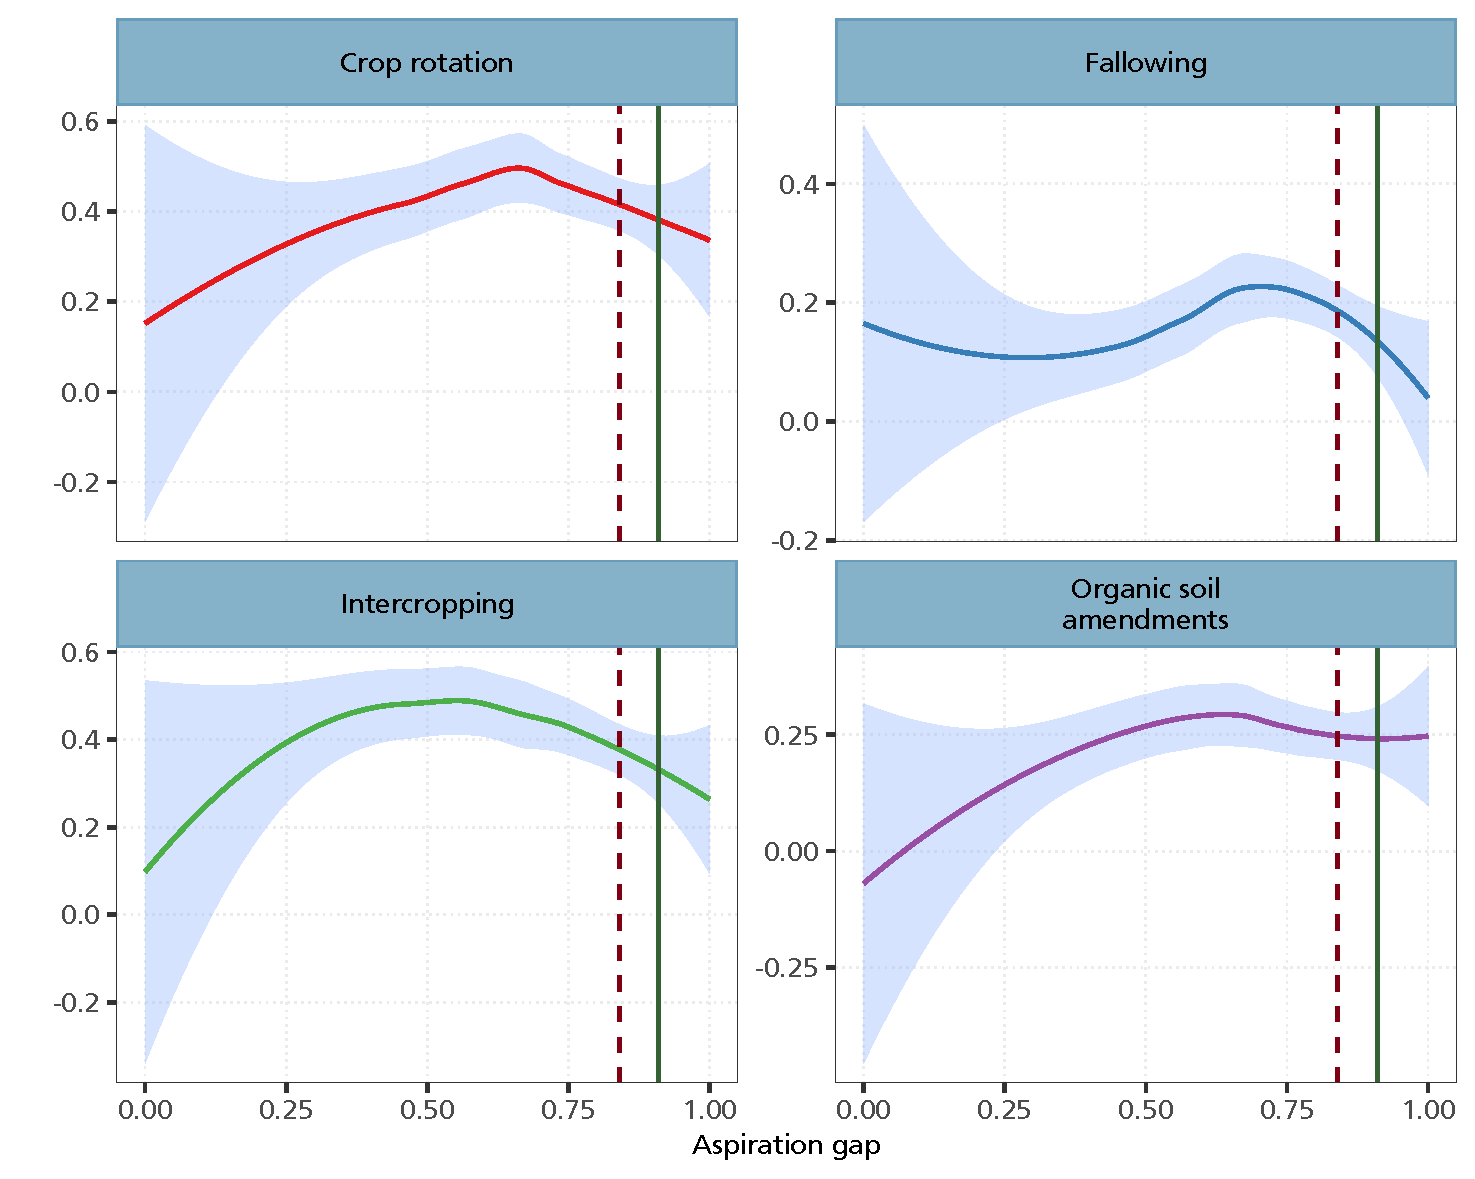
\includegraphics[width=\textwidth]{figures/fig_NP_ken.pdf}

\caption*{
Note: The graph illustrates the relationship between the variable CSA and Aspiration Gap, stratified by the four different practices for Kenya.The solid line on each plot depicts a Loess smoothed relationship between aspiration gap and CSA practices. Loess smoothing is a nonparametric method that uses local weighted regression to fit a smooth curve through points in a scatter plot. This line represents the trend of CSA adoption as aspiration gap changes. The shaded region around the Loess line represents 95\% Confidence intervals. The red dashed line indicates the 75th percentile, and the green line represents the 90th percentile of the aspiration gap. This figure is derived from a locally weighted regression analysis with a span (alpha) of 0.8 and a polynomial degree of 0. 
}
\end{figure}
\newpage

\hypertarget{cross-country-heterogeneity}{%
\section{Cross country heterogeneity}\label{cross-country-heterogeneity}}

\begin{landscape}\begingroup\fontsize{7}{9}\selectfont

\begin{ThreePartTable}
\begin{TableNotes}[para]
\item \textit{Note: } 
\item The table presents the results of OLS regressions between aspirations failure and CSA practices by country.Robust standard errors are in brackates. The statistical tests conducted are two-sided t-tests. P-values is denoted in square brackets. The presence of an asterisk (*) above a coefficient indicates that the coefficient is statistically different from zero at a predetermined level of significance (*** p<0.01, ** p<0.05, * p<0.1). All regressions include a comprehensive set of village fixed effects to control for potential unobserved heterogeneity.
\end{TableNotes}
\begin{longtable}[t]{lrrrrlrrr}
\caption{\label{tab:unnamed-chunk-10} Full OLS estimates of the relationship between aspirations and CSA practices by country}\\
\toprule
\multicolumn{1}{c}{ } & \multicolumn{4}{c}{Cameroon} & \multicolumn{4}{c}{Kenya} \\
\cmidrule(l{3pt}r{3pt}){2-5} \cmidrule(l{3pt}r{3pt}){6-9}
variables & Crop rotation (1/0) & Intercropping (1/0) & Fallowing (1/0) & Organic soil amendments (1/0) & Crop rotation (1/0) & Intercropping (1/0) & Fallowing (1/0) & Organic soil amendments (1/0)\\
\midrule
\endfirsthead
\caption[]{\label{tab:unnamed-chunk-10} Full OLS estimates of the relationship between aspirations and CSA practices by country \textit{(continued)}}\\
\toprule
variables & Crop rotation (1/0) & Intercropping (1/0) & Fallowing (1/0) & Organic soil amendments (1/0) & Crop rotation (1/0) & Intercropping (1/0) & Fallowing (1/0) & Organic soil amendments (1/0)\\
\midrule
\endhead

\endfoot
\bottomrule
\insertTableNotes
\endlastfoot
Aspirations & 0.024** & -0.019 & 0.007 & 0.022* & 0.021 & -0.007 & -0.001 & 0.045\\
 & (0.010) & (0.016) & (0.009) & (0.012) & (0.034) & (0.038) & (0.023) & (0.035)\\
 & {}[0.024] & {}[0.241] & {}[0.457] & {}[0.081] & {}[0.535] & {}[0.856] & {}[0.981] & {}[0.207]\\
Off-farm activity (1\/0) & 0.025 & -0.068 & -0.027 & -0.044 & 0.059 & -0.024 & 0.094** & 0.002\\
 & (0.057) & (0.055) & (0.045) & (0.044) & (0.048) & (0.051) & (0.045) & (0.047)\\
 & {}[0.661] & {}[0.226] & {}[0.549] & {}[0.324] & {}[0.231] & {}[0.645] & {}[0.045] & {}[0.969]\\
Household size (num) & 0.003 & -0.001 & 0.002 & 0.001 & 0.013 & 0.011 & 0.001 & 0.002\\
 & (0.004) & (0.004) & (0.004) & (0.005) & (0.008) & (0.009) & (0.007) & (0.008)\\
 & {}[0.508] & {}[0.878] & {}[0.678] & {}[0.852] & {}[0.138] & {}[0.245] & {}[0.913] & {}[0.838]\\
Credit access (1\/0) & 0.122** & 0.032 & 0.121** & 0.016 & 0.120** & 0.078* & -0.019 & 0.014\\
 & (0.057) & (0.040) & (0.053) & (0.064) & (0.049) & (0.043) & (0.032) & (0.042)\\
 & {}[0.038] & {}[0.428] & {}[0.030] & {}[0.798] & {}[0.020] & {}[0.081] & {}[0.554] & {}[0.730]\\
Age of head (years) & -0.000 & -0.002 & -0.002 & -0.003 & 0.001 & 0.002 & 0.000 & 0.000\\
 & (0.001) & (0.002) & (0.001) & (0.002) & (0.002) & (0.002) & (0.002) & (0.002)\\
 & {}[0.797] & {}[0.147] & {}[0.159] & {}[0.120] & {}[0.580] & {}[0.339] & {}[0.779] & {}[0.943]\\
Educational level (years) & 0.000 & 0.004 & 0.003 & -0.007 & -0.003 & -0.006 & -0.010** & -0.003\\
 & (0.005) & (0.007) & (0.005) & (0.006) & (0.007) & (0.006) & (0.005) & (0.005)\\
 & {}[0.986] & {}[0.602] & {}[0.591] & {}[0.236] & {}[0.649] & {}[0.316] & {}[0.040] & {}[0.472]\\
Cooperative membership (1\/0) & 0.009 & 0.042 & 0.068 & 0.090* & 0.085 & -0.015 & 0.027 & -0.034\\
 & (0.049) & (0.040) & (0.050) & (0.050) & (0.057) & (0.058) & (0.042) & (0.051)\\
 & {}[0.852] & {}[0.299] & {}[0.185] & {}[0.082] & {}[0.149] & {}[0.803] & {}[0.518] & {}[0.507]\\
Extension access (1\/0) & -0.005 & 0.041 & -0.068 & -0.057 & 0.161*** & 0.114** & 0.044 & 0.118***\\
 & (0.060) & (0.059) & (0.049) & (0.042) & (0.059) & (0.048) & (0.046) & (0.036)\\
 & {}[0.931] & {}[0.487] & {}[0.180] & {}[0.184] & {}[0.010] & {}[0.024] & {}[0.340] & {}[0.002]\\
Head is male (1\/0) & -0.001 & -0.031 & -0.039 & -0.050 & 0.031 & 0.030 & 0.032 & 0.087*\\
 & (0.042) & (0.055) & (0.034) & (0.037) & (0.045) & (0.052) & (0.043) & (0.045)\\
 & {}[0.980] & {}[0.571] & {}[0.260] & {}[0.186] & {}[0.491] & {}[0.573] & {}[0.465] & {}[0.059]\\
Asset index & 0.043** & -0.083*** & 0.045** & 0.060*** & 0.022 & 0.044** & 0.033** & 0.005\\
 & (0.018) & (0.022) & (0.018) & (0.021) & (0.017) & (0.018) & (0.015) & (0.016)\\
 & {}[0.026] & {}[0.001] & {}[0.018] & {}[0.006] & {}[0.194] & {}[0.020] & {}[0.035] & {}[0.776]\\
Observations & 582 & 582 & 582 & 582 & 530 & 530 & 530 & 530\\
R-squared & 0.311 & 0.189 & 0.315 & 0.323 & 0.282 & 0.307 & 0.125 & 0.114\\
Additional controls & Yes & Yes & Yes & Yes & Yes & Yes & Yes & Yes\\
Village FE & No & No & No & No & Yes & Yes & Yes & Yes\\
F test & 2.215 & 4.160 & 2.803 & 2.433 & 7.010 & 4.657 & 2.372 & 3.224\\*
\end{longtable}
\end{ThreePartTable}
\endgroup{}
\end{landscape}

\newpage

\begin{landscape}\begingroup\fontsize{7}{9}\selectfont

\begin{ThreePartTable}
\begin{TableNotes}[para]
\item \textit{Note: } 
\item The table presents the results of OLS regressions between aspirations failure and CSA practices by country.Robust standard errors are in brackates. The statistical tests conducted are two-sided t-tests. P-values is denoted in square brackets. The presence of an asterisk (*) above a coefficient indicates that the coefficient is statistically different from zero at a predetermined level of significance (*** p<0.01, ** p<0.05, * p<0.1). All regressions include a comprehensive set of district fixed effects to control for potential unobserved heterogeneity.
\end{TableNotes}
\begin{longtable}[t]{lrrrrlrrr}
\caption{\label{tab:unnamed-chunk-11} Full OLS estimates of the relationship between aspirations failure and CSA practices by country}\\
\toprule
\multicolumn{1}{c}{ } & \multicolumn{4}{c}{Cameroon} & \multicolumn{4}{c}{Kenya} \\
\cmidrule(l{3pt}r{3pt}){2-5} \cmidrule(l{3pt}r{3pt}){6-9}
variables & Crop rotation (1/0) & Intercropping (1/0) & Fallowing (1/0) & Organic soil amendments (1/0) & Crop rotation (1/0) & Intercropping (1/0) & Fallowing (1/0) & Organic soil amendments (1/0)\\
\midrule
\endfirsthead
\caption[]{\label{tab:unnamed-chunk-11} Full OLS estimates of the relationship between aspirations failure and CSA practices by country \textit{(continued)}}\\
\toprule
variables & Crop rotation (1/0) & Intercropping (1/0) & Fallowing (1/0) & Organic soil amendments (1/0) & Crop rotation (1/0) & Intercropping (1/0) & Fallowing (1/0) & Organic soil amendments (1/0)\\
\midrule
\endhead

\endfoot
\bottomrule
\insertTableNotes
\endlastfoot
Aspiration gap (0-1) & 0.510 & 1.127*** & 0.677** & 0.364 & 0.916* & 0.897 & 0.555 & 0.717\\
 & (0.304) & (0.375) & (0.311) & (0.288) & (0.529) & (0.544) & (0.431) & (0.565)\\
 & {}[0.102] & {}[0.005] & {}[0.037] & {}[0.214] & {}[0.092] & {}[0.108] & {}[0.206] & {}[0.213]\\
Gap squared (0-1) & -0.494 & -1.138*** & -0.667** & -0.301 & -0.654 & -0.807* & -0.346 & -0.515\\
 & (0.295) & (0.333) & (0.296) & (0.252) & (0.437) & (0.454) & (0.310) & (0.480)\\
 & {}[0.103] & {}[0.002] & {}[0.031] & {}[0.240] & {}[0.143] & {}[0.084] & {}[0.272] & {}[0.291]\\
Off-farm activity (1\/0) & 0.028 & -0.071 & -0.026 & -0.042 & 0.067 & -0.035 & 0.106** & 0.006\\
 & (0.057) & (0.054) & (0.047) & (0.044) & (0.048) & (0.049) & (0.049) & (0.048)\\
 & {}[0.621] & {}[0.195] & {}[0.579] & {}[0.347] & {}[0.178] & {}[0.486] & {}[0.037] & {}[0.903]\\
Household size (num) & 0.003 & 0.000 & 0.002 & 0.001 & 0.013 & 0.010 & 0.001 & 0.002\\
 & (0.004) & (0.004) & (0.004) & (0.005) & (0.008) & (0.009) & (0.007) & (0.008)\\
 & {}[0.421] & {}[0.966] & {}[0.587] & {}[0.799] & {}[0.124] & {}[0.264] & {}[0.842] & {}[0.821]\\
Credit access (1\/0) & 0.119** & 0.030 & 0.118** & 0.013 & 0.118** & 0.077* & -0.019 & 0.012\\
 & (0.056) & (0.039) & (0.053) & (0.065) & (0.050) & (0.044) & (0.031) & (0.043)\\
 & {}[0.041] & {}[0.460] & {}[0.035] & {}[0.838] & {}[0.023] & {}[0.093] & {}[0.542] & {}[0.789]\\
Age of head (years) & -0.001 & -0.002 & -0.002 & -0.003 & 0.001 & 0.002 & 0.001 & 0.000\\
 & (0.001) & (0.001) & (0.001) & (0.002) & (0.002) & (0.002) & (0.002) & (0.002)\\
 & {}[0.702] & {}[0.128] & {}[0.123] & {}[0.106] & {}[0.527] & {}[0.373] & {}[0.652] & {}[0.973]\\
Educational level (years) & -0.001 & 0.002 & 0.001 & -0.008 & -0.001 & -0.006 & -0.010** & -0.000\\
 & (0.005) & (0.007) & (0.005) & (0.006) & (0.006) & (0.006) & (0.005) & (0.005)\\
 & {}[0.913] & {}[0.830] & {}[0.766] & {}[0.211] & {}[0.860] & {}[0.325] & {}[0.046] & {}[0.939]\\
Cooperative membership (1\/0) & -0.001 & 0.013 & 0.052 & 0.086* & 0.085 & -0.016 & 0.029 & -0.036\\
 & (0.049) & (0.040) & (0.046) & (0.050) & (0.059) & (0.057) & (0.041) & (0.052)\\
 & {}[0.989] & {}[0.750] & {}[0.260] & {}[0.091] & {}[0.158] & {}[0.778] & {}[0.478] & {}[0.494]\\
Extension access (1\/0) & -0.012 & 0.037 & -0.073 & -0.061 & 0.159** & 0.119** & 0.037 & 0.123***\\
 & (0.060) & (0.057) & (0.050) & (0.043) & (0.059) & (0.050) & (0.043) & (0.036)\\
 & {}[0.846] & {}[0.524] & {}[0.152] & {}[0.162] & {}[0.011] & {}[0.022] & {}[0.396] & {}[0.002]\\
Head is male (1\/0) & 0.004 & -0.036 & -0.038 & -0.045 & 0.023 & 0.019 & 0.027 & 0.082*\\
 & (0.043) & (0.055) & (0.035) & (0.036) & (0.045) & (0.052) & (0.041) & (0.045)\\
 & {}[0.935] & {}[0.518] & {}[0.280] & {}[0.217] & {}[0.611] & {}[0.717] & {}[0.510] & {}[0.081]\\
Asset index & 0.051*** & -0.078*** & 0.051*** & 0.066*** & 0.024 & 0.039** & 0.033** & 0.011\\
 & (0.018) & (0.020) & (0.018) & (0.020) & (0.016) & (0.017) & (0.014) & (0.016)\\
 & {}[0.007] & {}[0.000] & {}[0.009] & {}[0.002] & {}[0.142] & {}[0.029] & {}[0.030] & {}[0.506]\\
Observations & 582 & 582 & 582 & 582 & 530 & 530 & 530 & 530\\
R-squared & 0.311 & 0.216 & 0.324 & 0.320 & 0.286 & 0.313 & 0.130 & 0.112\\
F test & 2.570 & 4.618 & 3.005 & 2.023 & 6.858 & 5.829 & 2.632 & 3.818\\*
\end{longtable}
\end{ThreePartTable}
\endgroup{}
\end{landscape}
\newpage

\newpage

\hypertarget{mvp-of-the-relationship-between-aspirations-aspiration-failures-and-csa-practices}{%
\section{MVP of the relationship between aspirations, aspiration failures and CSA practices}\label{mvp-of-the-relationship-between-aspirations-aspiration-failures-and-csa-practices}}

\begin{landscape}\begingroup\fontsize{7}{9}\selectfont

\begin{ThreePartTable}
\begin{TableNotes}[para]
\item \textit{Note: } 
\item This table displays the findings of Multivariate Probit (MVP) regressions, applied to investigate the relationship between aspiration and the adoption of Climate-Smart Agriculture (CSA) practices. Robust standard errors are reported in brackets to control for potential heteroscedasticity. Two-sided t-tests were conducted for the statistical tests, and corresponding p-values are noted within square brackets. Coefficients denoted with an asterisk () represent statistical significance at pre-established levels (** p<0.01, ** p<0.05, * p<0.1). To account for potential unobserved heterogeneity, all regressions incorporate a comprehensive set of village fixed effects.
\end{TableNotes}
\begin{longtable}[t]{lrrrr}
\caption{\label{tab:unnamed-chunk-13}MVP of the relationship between aspirations and CSA practices}\\
\toprule
variables & Crop rotation (1/0) & Intercropping (1/0) & Fallowing (1/0) & Organic soil amendments (1/0)\\
\midrule
\endfirsthead
\caption[]{\label{tab:unnamed-chunk-13}MVP of the relationship between aspirations and CSA practices \textit{(continued)}}\\
\toprule
variables & Crop rotation (1/0) & Intercropping (1/0) & Fallowing (1/0) & Organic soil amendments (1/0)\\
\midrule
\endhead

\endfoot
\bottomrule
\insertTableNotes
\endlastfoot
Aspirations & 0.216*** & -0.0594 & 0.0462 & 0.125***\\
 & (0.0370) & (0.0421) & (0.0302) & (0.0470)\\
Off-farm activity (1\/0) & -0.0803 & -0.155 & 0.0792 & -0.140\\
 & (0.103) & (0.117) & (0.126) & (0.111)\\
Household size (num) & 0.0135 & 0.0151 & 0.00975 & 0.00650\\
 & (0.0139) & (0.0137) & (0.0145) & (0.0142)\\
Credit access (1\/0) & 0.224** & 0.209** & 0.0750 & 0.000383\\
 & (0.0997) & (0.0986) & (0.115) & (0.114)\\
Age of head (years) & 0.00227 & 0.000528 & -0.000785 & -0.00565\\
 & (0.00301) & (0.00399) & (0.00396) & (0.00440)\\
Educational level (years) & -0.0129 & 0.00122 & -0.0274* & -0.0179\\
 & (0.0119) & (0.0143) & (0.0145) & (0.0136)\\
Cooperative membership (1\/0) & 0.264** & 0.0867 & 0.227* & 0.0815\\
 & (0.105) & (0.112) & (0.126) & (0.112)\\
Extension access (1\/0) & 0.284** & 0.228* & -0.0331 & 0.148\\
 & (0.119) & (0.121) & (0.126) & (0.0988)\\
Head is male (1\/0) & 0.0140 & 0.0871 & -0.0357 & 0.0258\\
 & (0.0823) & (0.117) & (0.110) & (0.115)\\
Asset index & 0.0826** & -0.0349 & 0.163*** & 0.106***\\
 & (0.0324) & (0.0481) & (0.0429) & (0.0389)\\
Constant & -2.734*** & 0.962 & -0.266 & -1.510**\\
 & (0.511) & (0.695) & (0.547) & (0.701)\\
\midrule
Observations & 1,112 & 1,112 & 1,112 & 1,112\\
Additional controls & Yes & Yes & Yes & Yes\\
Village FE & Yes & Yes & Yes & Yes\\
Year FE & Yes & Yes & Yes & Yes\\
\midrule
\_ & Coefficent & Std. Err. &  & \\
\midrule
atanhrho-12 & -0.0102 & (0.0785) &  & \\
atanhrho-13 & 0.491*** & (0.0989) &  & \\
atanhrho-14 & 0.324*** & (0.0855) &  & \\
atanhrho-23 & 0.186* & (0.0996) &  & \\
atanhrho-24 & 0.217** & (0.0844) &  & \\
atanhrho-34 & 0.173* & (0.0929) &  & \\
\midrule
Robust standard errors in parentheses &  &  &  & \\
*** p<0.01, ** p<0.05, * p<0.1 &  &  &  & \\*
\end{longtable}
\end{ThreePartTable}
\endgroup{}
\end{landscape}
\newpage

\begin{landscape}\begingroup\fontsize{7}{9}\selectfont

\begin{ThreePartTable}
\begin{TableNotes}[para]
\item \textit{Note: } 
\item The table displays the findings of Multivariate Probit (MVP) regressions, applied to investigate the relationship between aspiration failure and the adoption of Climate-Smart Agriculture (CSA) practices. Robust standard errors are reported in brackets to control for potential heteroscedasticity. Two-sided t-tests were conducted for the statistical tests, and corresponding p-values are noted within square brackets. Coefficients denoted with an asterisk () represent statistical significance at pre-established levels (** p<0.01, ** p<0.05, * p<0.1). To account for potential unobserved heterogeneity, all regressions incorporate a comprehensive set of village fixed effects.
\end{TableNotes}
\begin{longtable}[t]{lrrrr}
\caption{\label{tab:unnamed-chunk-14}MVP of the relationship between aspiration failure and CSA practices}\\
\toprule
variables & Crop rotation (1/0) & Intercropping (1/0) & Fallowing (1/0) & Organic soil amendments (1/0)\\
\midrule
\endfirsthead
\caption[]{\label{tab:unnamed-chunk-14}MVP of the relationship between aspiration failure and CSA practices \textit{(continued)}}\\
\toprule
variables & Crop rotation (1/0) & Intercropping (1/0) & Fallowing (1/0) & Organic soil amendments (1/0)\\
\midrule
\endhead

\endfoot
\bottomrule
\insertTableNotes
\endlastfoot
Aspiration gap (0-1) & 0.373 & 3.829*** & 1.783** & 1.429\\
 & (0.879) & (0.972) & (0.903) & (1.040)\\
Gap squared (0-1) & 0.125 & -3.805*** & -1.413* & -0.910\\
 & (0.776) & (0.887) & (0.747) & (0.850)\\
Off-farm activity (1\/0) & -0.0336 & -0.210* & 0.0802 & -0.126\\
 & (0.103) & (0.118) & (0.128) & (0.110)\\
Household size (num) & 0.00890 & 0.0163 & 0.00903 & 0.00687\\
 & (0.0125) & (0.0130) & (0.0146) & (0.0138)\\
Credit access (1\/0) & 0.0707 & 0.216** & 0.0350 & -0.0348\\
 & (0.105) & (0.105) & (0.114) & (0.114)\\
Age of head (years) & 0.00438 & 0.000192 & -0.000128 & -0.00549\\
 & (0.00308) & (0.00398) & (0.00393) & (0.00427)\\
Educational level (years) & 0.0160 & -0.00313 & -0.0207 & -0.00972\\
 & (0.0114) & (0.0148) & (0.0141) & (0.0131)\\
Cooperative membership (1\/0) & 0.289*** & 0.0240 & 0.212* & 0.0859\\
 & (0.107) & (0.112) & (0.122) & (0.110)\\
Extension access (1\/0) & 0.240** & 0.256** & -0.0394 & 0.138\\
 & (0.118) & (0.123) & (0.125) & (0.0960)\\
Head is male (1\/0) & 0.0292 & 0.0462 & -0.0454 & 0.0355\\
 & (0.0878) & (0.122) & (0.111) & (0.113)\\
Asset index & 0.110*** & -0.0445 & 0.168*** & 0.125***\\
 & (0.0305) & (0.0449) & (0.0417) & (0.0369)\\
Constant & -0.732** & -0.410 & -0.305 & -0.506\\
 & (0.348) & (0.406) & (0.436) & (0.486)\\
\midrule
Observations & 1,112 & 1,112 & 1,112 & 1,112\\
Additional controls & Yes & Yes & Yes & Yes\\
Village FE & Yes & Yes & Yes & Yes\\
Year FE & Yes & Yes & Yes & Yes\\
\midrule
\_ & Coefficent & Std. Err. &  & \\
\midrule
atanhrho-12 & -0.0154 & (0.0822) &  & \\
atanhrho-13 & 0.487*** & (0.0988) &  & \\
atanhrho-14 & 0.330*** & (0.0871) &  & \\
atanhrho-23 & 0.173* & (0.101) &  & \\
atanhrho-24 & 0.209** & (0.0852) &  & \\
atanhrho-34 & 0.170* & (0.0924) &  & \\
\midrule
Robust standard errors in parentheses &  &  &  & \\
*** p<0.01, ** p<0.05, * p<0.1 &  &  &  & \\*
\end{longtable}
\end{ThreePartTable}
\endgroup{}
\end{landscape}

\hypertarget{robustness-checks}{%
\section{Robustness Checks}\label{robustness-checks}}

\newpage

\begin{landscape}\begingroup\fontsize{7}{9}\selectfont

\begin{ThreePartTable}
\begin{TableNotes}[para]
\item \textit{Note: } 
\item The table provides the findings from Full Poisson and Ordered probit estimations, carried out to explore the association between aspiration and Climate-Smart Agriculture (CSA) practices. The Full Poisson model was utilized to handle count outcomes while the Ordered probit model was used for ordinal outcomes. Robust standard errors, stated within brackets, were utilized to mitigate the impact of heteroscedasticity. Statistical tests were performed using two-sided t-tests, and the corresponding p-values are displayed within square brackets. Coefficients designated with an asterisk () indicate statistical significance at preset significance thresholds (** p<0.01, ** p<0.05, * p<0.1). 
\end{TableNotes}
\begin{longtable}[t]{lrrrrlr}
\caption{\label{tab:unnamed-chunk-15} Full Poisson and Ordered probit estimates of the relationship between aspiration and CSA practices }\\
\toprule
\multicolumn{1}{c}{ } & \multicolumn{3}{c}{POISSON} & \multicolumn{3}{c}{ORDERED PROBIT} \\
\cmidrule(l{3pt}r{3pt}){2-4} \cmidrule(l{3pt}r{3pt}){5-7}
variable & (1) & (2) & (3) & (1) & (2) & (3)\\
\midrule
\endfirsthead
\caption[]{\label{tab:unnamed-chunk-15} Full Poisson and Ordered probit estimates of the relationship between aspiration and CSA practices  \textit{(continued)}}\\
\toprule
variable & (1) & (2) & (3) & (1) & (2) & (3)\\
\midrule
\endhead

\endfoot
\bottomrule
\insertTableNotes
\endlastfoot
Aspirations & 0.131*** & 0.124*** & 0.021 & 0.210*** & 0.202*** & 0.039\\
 & (0.019) & (0.018) & (0.014) & (0.031) & (0.030) & (0.028)\\
 & {}[0.000] & {}[0.000] & {}[0.141] & {}[0.000] & {}[0.000] & {}[0.164]\\
Off-farm activity &  & -0.024 & -0.013 &  & -0.025 & 0.010\\
 &  & (0.040) & (0.042) &  & (0.067) & (0.084)\\
 &  & {}[0.557] & {}[0.756] &  & {}[0.709] & {}[0.906]\\
Household size &  & 0.005 & 0.007 &  & 0.008 & 0.017\\
 &  & (0.005) & (0.005) &  & (0.010) & (0.012)\\
 &  & {}[0.381] & {}[0.174] &  & {}[0.418] & {}[0.143]\\
Credit access &  & 0.024 & 0.128*** &  & 0.031 & 0.254***\\
 &  & (0.045) & (0.044) &  & (0.075) & (0.085)\\
 &  & {}[0.599] & {}[0.003] &  & {}[0.680] & {}[0.003]\\
Age of head &  & 0.005*** & -0.001 &  & 0.009*** & -0.002\\
 &  & (0.002) & (0.002) &  & (0.003) & (0.003)\\
 &  & {}[0.003] & {}[0.606] &  & {}[0.002] & {}[0.548]\\
Educational level &  & 0.002 & -0.005 &  & 0.005 & -0.012\\
 &  & (0.006) & (0.006) &  & (0.011) & (0.012)\\
 &  & {}[0.723] & {}[0.404] &  & {}[0.636] & {}[0.319]\\
Cooperative membership &  & 0.035 & 0.074** &  & 0.056 & 0.155**\\
 &  & (0.042) & (0.038) &  & (0.074) & (0.077)\\
 &  & {}[0.409] & {}[0.048] &  & {}[0.452] & {}[0.044]\\
Extension access &  & 0.083* & 0.106** &  & 0.131 & 0.201**\\
 &  & (0.048) & (0.051) &  & (0.084) & (0.102)\\
 &  & {}[0.081] & {}[0.040] &  & {}[0.119] & {}[0.049]\\
Head is male &  & -0.006 & 0.017 &  & -0.029 & 0.016\\
 &  & (0.048) & (0.040) &  & (0.082) & (0.077)\\
 &  & {}[0.895] & {}[0.671] &  & {}[0.720] & {}[0.833]\\
Asset index &  & 0.047*** & 0.051*** &  & 0.097*** & 0.108***\\
 &  & (0.014) & (0.017) &  & (0.026) & (0.036)\\
 &  & {}[0.001] & {}[0.003] &  & {}[0.000] & {}[0.002]\\
Observations & 1,112 & 1,112 & 1,112 & 1,112 & 1,112 & 1,112\\
Additional controls & No & Yes & Yes & No & Yes & Yes\\
Village FE & No & No & Yes & No & No & Yes\\*
\end{longtable}
\end{ThreePartTable}
\endgroup{}
\end{landscape}
\newpage

\begin{landscape}\begingroup\fontsize{7}{9}\selectfont

\begin{ThreePartTable}
\begin{TableNotes}[para]
\item \textit{Note: } 
\item The table provides the findings from Full Poisson and Ordered probit estimations, carried out to explore the association between aspiration failure and Climate-Smart Agriculture (CSA) practices. The Full Poisson model was utilized to handle count outcomes while the Ordered probit model was used for ordinal outcomes. Robust standard errors, stated within brackets, were utilized to mitigate the impact of heteroscedasticity. Statistical tests were performed using two-sided t-tests, and the corresponding p-values are displayed within square brackets. Coefficients designated with an asterisk () indicate statistical significance at preset significance thresholds (** p<0.01, ** p<0.05, * p<0.1).
\end{TableNotes}
\begin{longtable}[t]{lrr}
\caption{\label{tab:unnamed-chunk-16}Full Poisson and Ordered probit estimates of the relationship between aspiration filure and CSA practices}\\
\toprule
\multicolumn{1}{c}{ } & \multicolumn{1}{c}{POISSON} & \multicolumn{1}{c}{ORDERED PROBIT} \\
\cmidrule(l{3pt}r{3pt}){2-2} \cmidrule(l{3pt}r{3pt}){3-3}
variables & (1) & (2)\\
\midrule
\endfirsthead
\caption[]{\label{tab:unnamed-chunk-16}Full Poisson and Ordered probit estimates of the relationship between aspiration filure and CSA practices \textit{(continued)}}\\
\toprule
variables & (1) & (2)\\
\midrule
\endhead

\endfoot
\bottomrule
\insertTableNotes
\endlastfoot
Aspiration gap (0-1) & 1.729*** & 3.251***\\
 & (0.461) & (0.774)\\
 & {}[0.000] & {}[0.000]\\
Gap squared (0-1) & -1.493*** & -2.873***\\
 & (0.364) & (0.664)\\
 & {}[0.000] & {}[0.000]\\
Off-farm activity (1\/0) & -0.017 & -0.010\\
 & (0.042) & (0.086)\\
 & {}[0.677] & {}[0.909]\\
Household size (num) & 0.007 & 0.018\\
 & (0.005) & (0.012)\\
 & {}[0.129] & {}[0.116]\\
Credit access (1\/0) & 0.123*** & 0.247***\\
 & (0.044) & (0.089)\\
 & {}[0.005] & {}[0.005]\\
Age of head (years) & -0.001 & -0.003\\
 & (0.002) & (0.003)\\
 & {}[0.505] & {}[0.420]\\
Educational level (years) & -0.006 & -0.012\\
 & (0.006) & (0.013)\\
 & {}[0.351] & {}[0.325]\\
Cooperative membership (1\/0) & 0.055 & 0.121\\
 & (0.036) & (0.074)\\
 & {}[0.123] & {}[0.103]\\
Extension access (1\/0) & 0.107** & 0.214**\\
 & (0.052) & (0.105)\\
 & {}[0.041] & {}[0.041]\\
Head is male (1\/0) & 0.010 & -0.001\\
 & (0.039) & (0.077)\\
 & {}[0.804] & {}[0.984]\\
Asset index & 0.057*** & 0.116***\\
 & (0.016) & (0.033)\\
 & {}[0.000] & {}[0.000]\\
Observations & 1,112 & 1,112\\
Additional controls & Yes & Yes\\
Village FE & Yes & Yes\\*
\end{longtable}
\end{ThreePartTable}
\endgroup{}
\end{landscape}

\end{document}
